\documentclass[a4paper, article, oneside, USenglish, IN5460]{memoir}

%% Title page
\usepackage{style/projectfp} 


%% Encoding
\usepackage[utf8]{inputenx} % Source code
\usepackage[T1]{fontenc}    % PDF


%% Fonts and typography
\usepackage{lmodern}           % Latin Modern Roman
\usepackage[scaled]{beramono}  % Bera Mono (Bitstream Vera Sans Mono)
\renewcommand{\sfdefault}{phv} % Helvetica
\usepackage[final]{microtype}  % Improved typography
\renewcommand{\abstractnamefont}{\sffamily\bfseries}                 % Abstract
\renewcommand*{\chaptitlefont}{\Large\bfseries\sffamily\raggedright} % Chapter
\setsecheadstyle{\large\bfseries\sffamily\raggedright}               % Section
\setsubsecheadstyle{\large\bfseries\sffamily\raggedright}            % Subsection
\setsubsubsecheadstyle{\normalsize\bfseries\sffamily\raggedright}    % Subsubsection
\setparaheadstyle{\normalsize\bfseries\sffamily\raggedright}         % Paragraph
\setsubparaheadstyle{\normalsize\bfseries\sffamily\raggedright}      % Subparagraph

%% Mathematics
\usepackage{amssymb}   % Extra symbols
\usepackage{amsthm}    % Theorem-like environments
\usepackage{thmtools}  % Theorem-like environments
\usepackage{mathtools} % Fonts and environments for mathematical formuale
\usepackage{mathrsfs}  % Script font with \mathscr{}

\title{Appliance Energy Consumption Prediction and Classification Using Federated Learning}
\authors{F. Ofstad, Z. Shan, R. Syed, H. Zhang}

\addbibresource{bibliography.bib}

\begin{document}

\projectfrontpage


\chapter{Introducton}

The purpose of this report is to construct a Federated Learning model, which aggregates the resulting parameters from client models. The client models have two tasks:
\begin{enumerate}
    \item to train a model to predict the energy consumption for appliances in a household
    \item Train a model to classify the type of appliance based on their energy consumption.    
\end{enumerate}

To this end, we used the tensorflow package for Python when creating the client models using Keras, and the extension tensorflow federated for the aggregating model. The steps the program takes are as follows:
\section{Preprocess the data}
We first convert the provided excel file into csv files for each household. This is done to conceptually emulate FL as each client should only have access to their own data, and because CSV files are generally faster to load in python.

The clients themselves utilize LSTM and RNN models with n layers and n nodes #TODO Fill in

The federated model runs these clients and extracts the averaged weights which it used for the aggregated model.



\begin{figure}[h]
  \centering
    % This file was created with tikzplotlib v0.10.1.
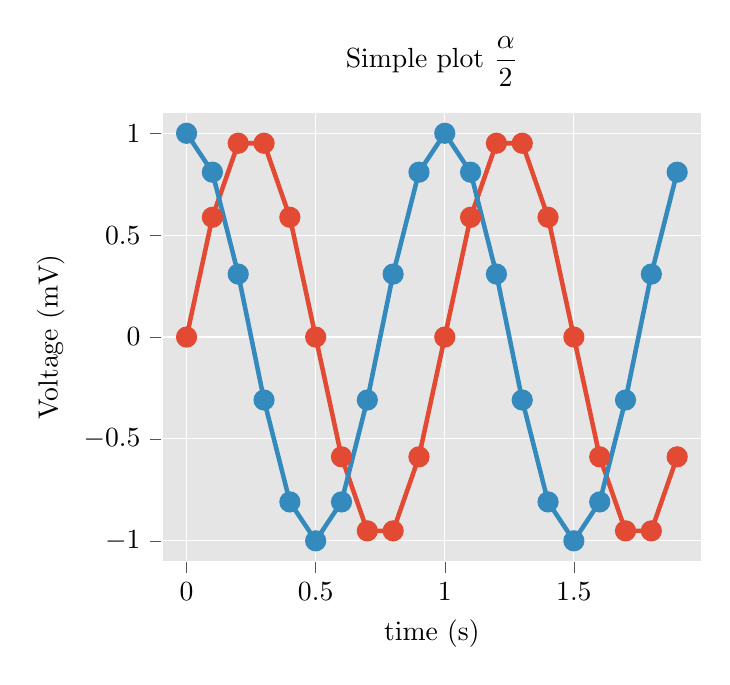
\begin{tikzpicture}

\definecolor{chocolate2267451}{RGB}{226,74,51}
\definecolor{dimgray85}{RGB}{85,85,85}
\definecolor{gainsboro229}{RGB}{229,229,229}
\definecolor{steelblue52138189}{RGB}{52,138,189}

\begin{axis}[
axis background/.style={fill=gainsboro229},
axis line style={white},
tick align=outside,
tick pos=left,
title={Simple plot \(\displaystyle \frac{\alpha}{2}\)},
x grid style={white},
xlabel={time (s)},
xmajorgrids,
xmin=-0.095, xmax=1.995,
xtick style={color=dimgray85},
y grid style={white},
ylabel={Voltage (mV)},
ymajorgrids,
ymin=-1.1, ymax=1.1,
ytick style={color=dimgray85}
]
\addplot [line width=1.64pt, chocolate2267451, mark=*, mark size=3, mark options={solid}]
table {%
0 0
0.1 0.587785252292473
0.2 0.951056516295154
0.3 0.951056516295154
0.4 0.587785252292473
0.5 1.22464679914735e-16
0.6 -0.587785252292473
0.7 -0.951056516295154
0.8 -0.951056516295154
0.9 -0.587785252292473
1 -2.44929359829471e-16
1.1 0.587785252292474
1.2 0.951056516295154
1.3 0.951056516295154
1.4 0.587785252292473
1.5 3.67394039744206e-16
1.6 -0.587785252292473
1.7 -0.951056516295154
1.8 -0.951056516295154
1.9 -0.587785252292473
};
\addplot [line width=1.64pt, steelblue52138189, mark=*, mark size=3, mark options={solid}]
table {%
0 1
0.1 0.809016994374947
0.2 0.309016994374947
0.3 -0.309016994374948
0.4 -0.809016994374947
0.5 -1
0.6 -0.809016994374947
0.7 -0.309016994374948
0.8 0.309016994374947
0.9 0.809016994374947
1 1
1.1 0.809016994374947
1.2 0.309016994374947
1.3 -0.309016994374947
1.4 -0.809016994374947
1.5 -1
1.6 -0.809016994374948
1.7 -0.309016994374946
1.8 0.309016994374947
1.9 0.809016994374947
};
\end{axis}

\end{tikzpicture}

  \caption{Test plot using tikzplotlib}
\end{figure}



\chapter{Question 1}

The following section tests the federated learning efficiency when predicting appliance energy consumption.

\section{Question 1.1}

\begin{figure}[h]
  \centering
    %\input{report/figures/training_error_1.1}
  \caption{Simulation plot of the training error in MSE}
\end{figure}

\begin{figure}[h]
  \centering
    %\input{report/figures/}
  \caption{Simulation plot comparing the predicted output with the ground truth for training}
\end{figure}

\begin{figure}[h]
  \centering
    %\input{report/figures/}
  \caption{Simulation plot comparing the predicted output with the ground truth for testing}
\end{figure}


%Is the federated learning efficient in this scenario of appliance energy consumption prediction? Please discuss whether the performance of model training can be improved by adding more epochs or through other configuration changes.


\section{Question 1.2}

The following models use the same configurations as the previous model, except the trainer uses LSTM instead of regular RNN.

 %Compare the performance with that of RNN regarding execution time and prediction error during the test.

\chapter{Question 2}

This section reports the results of the classification model: determining the types of application based on the daily consumption of an appliance.

\section{Question 2.1}

%Is the federated learning efficient in this scenario of appliance classification? Please use simulation plots to show the classification accuracy during the training process using training (or training and validation) data, and show the classification accuracy of the trained model using test data. Please discuss whether the accuracy during the training and testing can be improved by adding more epochs or through other configuration changes.

\section{Question 2.2}

%The accuracy in Question 2.1 manifests how the model works for all the appliance as a whole.You also need to show how the classification works for each appliance. To do so, you need to generate the confusion matrix of the classification result, both for the model training and testing. The confusion matrix should present the classification accuracy for each appliance.

\section{Question 2.3}

%Keep the same settings as in Question 2.1 and 2.2, except that you use LSTM when implementing federated learning. You then show the simulation plots as required in Question 2.1 and 2.2, and compare with the results when using RNN.

\chapter{Conclusion}

Why is it so hard to make intuitive code that just works?? Google, you're a multibillion dollar company.. please! 
\newpage

\nocite{tensorflow2015-whitepaper}
\nocite{dataset}

\printbibliography{}

\vspace*{10mm}
\end{document}